% SEGMENT OLP-0549-S01
\documentclass[../../../include/open-logic-section]{subfiles}

\begin{document}

\olfileid{sth}{ordinals}{idea}	
\olsection{ஒரு வரிசையெண்ணின் பொதுக் கருத்து}

இயல் எண்களை அவற்றின் வழக்கமான வரிசையில் எடுத்துக்கொள்ளுங்கள்:
\begin{center}
	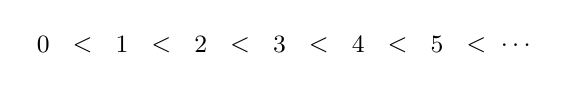
\begin{tikzpicture}
	\foreach \x/\xtext in {0, 1, 2, 3, 4, 5}
	{
		\node (\x a) at (\x, 1) {\small{$\x$}};
		\node (\x a) at (\x.5, 1) {\small{$<$}};
	}
	\node (ldots) at (6, 1) {\small{$\ldots$}};
	\end{tikzpicture}
\end{center}
தொழில்நுட்பச் சொல்லாட்சியில் இதை ஓர் $\omega$-தொடர் என்கிறோம். இந்தப்
பொது வரிசைப்படுத்தலே கணப் படிநிலை வரிசையின் நமது தொடக்கக் கட்டமைப்பிலும்
பிரதிபலிக்கிறது. ஆனால் இப்போது, மற்ற எல்லா எண்களுக்கும் பின்னால் வருமாறு
$0$ ஐ இந்தத் தொடரின் இறுதிக்கு நகர்த்துவதாகக் கொள்வோம்:
\begin{center}
	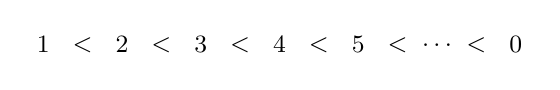
\begin{tikzpicture}
	\foreach \x/\xtext in {1, 2, 3, 4, 5}
	{
		\node (\x a) at (\x, 1) {\small{$\x$}};
		\node (\x a) at (\x.5, 1) {\small{$<$}};
	}
	\node (ldots) at (6, 1) {\small{$\ldots$}};
	\node (bea) at (6.5, 1) {\small{$<$}};
	\node (noa) at (7, 1) {\small{$0$}};
	\end{tikzpicture}
\end{center}
இங்குள்ள பொருள்கள் மாறவில்லை; ஆனால் அவை அடிப்படையிலேயே வேறுபட்ட முறையில்
வரிசைப்படுத்தப்பட்டுள்ளன: நமது முதல் வரிசைப்படுத்தலில் கடைசி உறுப்பு
இல்லை; புதிய வரிசைப்படுத்தலில் ஒன்று உள்ளது. உண்மையில், புதிய
வரிசைப்படுத்தலில் பொருள்களின் ஓர் $\omega$-தொடரைத் ($1, 2, 3, 4, 5,
\ldots$) தொடர்ந்து இன்னோர் உறுப்பு வருகிறது. அது ஓர்
$\omega+1$-தொடராக இருக்கும்.

இதே பொருள்களை மட்டும் பயன்படுத்தி, மேலும் பல வகையான வரிசைப்படுத்தல்களை
உருவாக்கலாம். எடுத்துக்காட்டாக, இயல்பான வரிசையிலுள்ள எல்லா இரட்டை
எண்களைத் தொடர்ந்து, இயல்பான வரிசையிலுள்ள எல்லா ஒற்றை எண்களும் வருவதாகக்
கொள்ளுங்கள்:
\begin{center}
	\begin{tikzpicture}
	\node(a1) at (1,1) {\small{$0$}};
	\node(a2) at (1.5,1) {\small{$<$}};
	\node(a3) at (2,1) {\small{$2$}};
	\node(a4) at (2.5,1) {\small{$<$}};
	\node(a5) at (3,1) {\small{$4$}};
	\node(a6) at (3.5,1) {\small{$<$}};
	\node(dots) at (4,1) {\small{$\ldots$}};
	\node(aaoe) at (4.5,1) {\small{$<$}};
	\node(b1) at (5,1) {\small{$1$}};
	\node(b2) at (5.5,1) {\small{$<$}};
	\node(b3) at (6,1) {\small{$3$}};
	\node(b4) at (6.5,1) {\small{$<$}};
	\node(b5) at (7,1) {\small{$\ldots$}};
	\end{tikzpicture}
\end{center}
இது ஓர் $\omega$-தொடரைத் தொடர்ந்து வரும் மற்றோர் $\omega$-தொடர்;
அதாவது ஓர் $\omega+\omega$-தொடர்.

இவ்வாறே நாம் தொடர்ந்து செல்லலாம். ஆனால் \emph{வரிசைப்படுத்தல்கள்} பற்றிய
இந்தப் பேச்சைப் பொதுவாகப் புரிந்துகொள்ள ஒரு வழியே நமக்குத் தேவை.

\end{document}
